\chapter{AsterixDB: Putting It All Together}
\label{ch:asterixdb}

\section{Overview}

Hyracks (Chapter~\ref{ch:hyracks}) and Algebricks (Chapter~\ref{ch:algebricks}) were developed in the context of the AsterixDB project, as mentioned in Chapter~\ref{ch:intro}. AsterixDB is a scalable Big-Data Management system built from the
ground up to ingest, manage, index, query, and analyze mass quantities semi-structured data~\cite{vision}. As a concluding case study, this chapter of the thesis describes
how Hyracks and Algebricks form the underpinnings of this Big-Data Management system. We begin by first providing an overview of AsterixDB's data definition capabilities (Section~\ref{ch:asterixdb:sec:ddl}) and its data manipulation capabilities (Section~\ref{ch:asterixdb:sec:dml}). In Section~\ref{ch:asterixdb:sec:sysarch}, we describe how Algebricks and Hyracks come together to form the bottom half of AsterixDB.

\section{Data Definition}
\label{ch:asterixdb:sec:ddl}

In this section we describe AsterixDB's data definition features.  We illustrate them by example through a scenario based on information about users and their messages from a hypothetical social network called Mugshot.com.

\subsection{Dataverses, Datatypes, and Datasets\label{ssec:dataverse}}

The top-level organizing concept in AsterixDB is the \emph{Dataverse}.
A Dataverse, short for "data universe", is a place (akin to a database in an RDBMS) within which one can create and manage the types, Datasets, functions, and other artifacts for a given application.
Initially, an AsterixDB instance contains no data other than the system catalogs, which live in a system-defined Dataverse (the Metadata Dataverse).
To store data in AsterixDB, one creates a Dataverse and then populates it with the desired Datatypes and Datasets.
A \emph{Datatype} specifies what its definer wants AsterixDB to know, a priori, about a kind of data that it will be asked to store.
A \emph{Dataset} is a stored collection of data instances of a Datatype, and one can define multiple Datasets of a given Datatype.
AsterixDB ensures that data inserted into a Dataset conforms to its specified type. 

Since AsterixDB targets semi-structured data, its data model provides the concept of \emph{open} (\emph{vs.~closed}) Datatypes.
When defining a type, the definer can use open Datatypes and tell AsterixDB as little or as much about their data up front as they wish.  
(The more AsterixDB knows about the potential residents of a Dataset, the less it needs to store in each individual data instance.)  
Instances of open Datatypes are allowed to have additional content, beyond what the type specifies, as long as they at least contain the information prescribed by the Datatype definition.  
Open types allow data to vary from one instance to another, leaving "wiggle room" for instance-level variations as well as for application evolution (in terms of what can be stored in the future). 
To restrict the objects in a Dataset to contain only what a Datatype says, with nothing extra in instances, one can opt to define a closed Datatype for that Dataset.
AsterixDB prevents users from storing objects with extra or illegally missing data in such a data set.
The closed, flat subset of ADM is thus relational.
Datatypes are open by default and closed only if their definition says so, the reason for this choice being that many Big Data analysts seem not to favor \emph{a priori} schema design and ADM's design targets semi-structured data.
To the best of our knowledge, this support for open and closed Datatypes is novel---we have not seen similarly flexible schema facilities in other data management systems, and it consistently garners very positive reactions when AsterixDB is presented to outside groups.

Shape-wise, ADM is a superset of JSON \cite{json}---ADM is what one gets by extending JSON with a larger set of Datatypes (e.g. datetime) and additional data modeling constructs (e.g. bags) drawn from object databases and then giving it a schema language.
We chose JSON for its self-describing nature, relative simplicity, and growing adoption in the Web world.
Note that, unlike AsterixDB, current JSON-based data platforms do not offer the option to define all (or part) of their data's schema.

%\begin{aql}[Data definition]{Dataverse and data types}{ddl:types}
\begin{ddl}[Dataverse and data types]{ddl:types}
drop dataverse TinySocial if exists;
create dataverse TinySocial;
use dataverse TinySocial;

create type EmploymentType as open {
    organization-name: string,
    start-date: date,
    end-date: date?
}

create type MugshotUserType as {
    id: int32,
    alias: string,
    name: string,
    user-since: datetime,
    address: {
        street: string,
        city: string,
        state: string,
        zip: string,
        country: string
    },
    friend-ids: {{ int32 }},
    employment: [EmploymentType]
}

create type MugshotMessageType as closed {
    message-id: int32,
    author-id: int32,
    timestamp: datetime,
    in-response-to: int32?,
    sender-location: point?,
    tags: {{ string }},
    message: string
}
\end{ddl}

We illustrate ADM by defining a Dataverse called \emph{TinySocial} to hold the Datatypes and Datasets for Mugshot.com.
The data definition statements in Data definition \ref{ddl:types} show how we can create the Dataverse and a set of ADM types to model Mugshot.com's users, their users' employment histories, and their messages. 
The first three lines tell AsterixDB to drop the old TinySocial Dataverse, if one exists, and to create a new Dataverse and make it the focus of the statements that follow. 
The first type creation statement creates a Datatype to hold information about one piece of a Mugshot user's employment history. 
It defines a record type with a mix of string and date data, much like a (flat) relational tuple.
Its first two fields are mandatory, with the last one (end-date) being optional as indicated by the "?" that follows it.
An optional field in ADM is like a nullable field in SQL -- it may be present or missing, but when present, its data type will conform to the Datatype's specification for it. Also, because EmploymentType is open, it is important to note that additional fields will be allowed at the instance level. 

\begin{table} [htbp]
\centering
\small
\begin{tabular}{|l|l|}
\hline %%%%%%%%%%%%%%%%%%%%%%%%%%%%%%%%%%%%%%%%%%%%%%%%%%%%%%%%
\textbf{Types}      & \textbf{functions}                     \\
\hline %%%%%%%%%%%%%%%%%%%%%%%%%%%%%%%%%%%%%%%%%%%%%%%%%%%%%%%%
string              & contains                               \\
                    & like                                   \\
                    & matches                                \\
                    & replace                                \\
                    & word-tokens                            \\
                    & edit-distance                          \\
                    & edit-distance-check                    \\
                    & edit-distance-contains                 \\
\hline %%%%%%%%%%%%%%%%%%%%%%%%%%%%%%%%%%%%%%%%%%%%%%%%%%%%%%%%
\emph{bag}          & similarity-jaccard                     \\
                    & similarity-jaccard-check               \\
\hline %%%%%%%%%%%%%%%%%%%%%%%%%%%%%%%%%%%%%%%%%%%%%%%%%%%%%%%%
date/time/datetime  & current-date/time/datetime             \\
interval            & interval-start-from-date/time/datetime \\
duration            & adjust-datetime-for-timezone           \\
day-time-duration   & adjust-time-for-timezone               \\
year-month-duration & subtract-date/time/datetime            \\
                    & interval-bin                           \\
                    & \emph{Allen's relations} on intervals  \\\hline %%%%%%%%%%%%%%%%%%%%%%%%%%%%%%%%%%%%%%%%%%%%%%%%%%%%%%%%
point               & spatial-distance                       \\
line                & spatial-area                           \\
rectangle           & spatial-intersect                      \\
circle              & spatial-cell                           \\
polygon             &                                        \\
\hline %%%%%%%%%%%%%%%%%%%%%%%%%%%%%%%%%%%%%%%%%%%%%%%%%%%%%%%%
\end{tabular}
\caption{Sample of advanced types and functions\label{tab:types}}
%\vspace{-0.1in}
\end{table}

The second create type statement creates a Datatype for Mugshot users.
MugshotUserType is also open since that is the default for AsterixDB Datatypes.
This second type highlights several additional features of ADM.
The address field illustrates one way that ADM is richer than the relational model; it holds a nested record containing the primary address of a user.
The friend-ids field shows another extension of ADM over the relational model and also over JSON.
This field holds a bag (unordered list) of integers -- presumably the Mugshot user ids for this user's friends.
Lastly for this type, its employment field is an ordered list of employment records, again a beyond-flat-relational structure.

The last create type statement in the example defines a Datatype to store the content of a Mugshot message.
In this case, since the type definition for Mugshot messages says \emph{closed}, the fields that it lists will be the only fields that instances of this type will be allowed to contain in Datasets of this type.
Also, among those fields, in-response-to and sender-location are optional, while the rest must be present in valid instances of the type.

Recall that AsterixDB aims to store and query not just Big Data, but Big \emph{Semi-structured} Data. 
Most of the fields in the create type statements above could be omitted, if desired, while changing only two things in terms of the example.  
One change would be the size of the data on disk. 
AsterixDB stores information about the fields defined \emph{a priori} as separate metadata; information about fields that are "just there" in instances of open Datatypes is stored within each instance.
A logical change would be that AsterixDB would be more flexible about the contents of records in the resulting Datasets, as it enforces only the specified details of the Datatype associated with a given Dataset.
The only fields that must currently be specified \emph{a priori} are the primary key fields. 

One other important feature of AsterixDB for managing today's Big Data is its built-in support for useful advanced primitive types and functions, specifically those related to space, time, and text.
Table \ref{tab:types} lists some of the advanced ADM primitive types as well as some of their corresponding AQL functions.
A complete list and more details can be found in the AsterixDB documentation \cite{docs}.

%spatial
%contructors (from coordinates or from string)
%accessors (get-x, get-y, get-points, get-center, get-radius)
%spatial-distance (between points)
%spatial-area (rectangle, circle, or polygon)
%spatial-intersect (2 spatial objects)
%spatial-cell

%constructors (from string)
%interval-from-date
%interval-from-time
%interval-from-datetime
%components (year/month/day/hour/minute/second/millisecond from data, time, datetime, duration)
%calendar-duration-from-datetime (normalize??)
%calendar-duration-from-date
%date-from-datetime, time-from-datetime
%date-from-unix-time-in-days, datetime-from-unix-time-in-ms, time-from-unix-time-in-ms
%get-interval-start, get-interval-end
%duration, year-month-duration, day-time-duration -> no functions?

\pagebreak
\subsection{Dataset and Index Creation}\label{ss:dataset}

Having defined our Datatypes, we can now proceed to create a pair of Datasets to store the actual data. 

\begin{ddl}[Datasets and indexes]{ddl:datasets}
create dataset MugshotUsers(MugshotUserType)
    primary key id;
create dataset MugshotMessages(MugshotMessageType)
    primary key message-id;

create index msUserSinceIdx 
    on MugshotUsers(user-since);
create index msTimestampIdx
    on MugshotMessages(timestamp);
create index msAuthorIdx
    on MugshotMessages(author-id) type btree;
create index msSenderLocIndex
    on MugshotMessages(sender-location) type rtree;
create index msMessageIdx
    on MugshotMessages(message) type keyword;
\end{ddl}

\eat{
use dataverse TinySocial;

load dataset MugshotUsers using localfs
(("path"="127.0.0.1:///Users/tillw/Documents/Papers/AsterixDB/703942dkdpdw/data/msu.adm.txt"),("format"="adm"));

load dataset MugshotMessages using localfs
(("path"="127.0.0.1:///Users/tillw/Documents/Papers/AsterixDB/703942dkdpdw/data/msm.adm.txt"),("format"="adm"));
}
\eat{
use dataverse TinySocial;

for $u in dataset MugshotUsers return $u;
for $m in dataset MugshotMessages return $m;
}

The two ADM DDL statements shown in Data definition \ref{ddl:datasets} will create Datasets to hold data in the TinySocial Dataverse.
The first creates a Dataset called MugshotUsers; 
this Dataset will store data conforming to MugshotUserType and has the id field as its primary key. 
The primary key is used by AsterixDB to uniquely identify instances for later lookup and for use in secondary indexes.
Each AsterixDB Dataset is stored (and indexed) as a B\textsuperscript{+}-tree keyed on primary key; secondary indexes point to indexed data by its primary key. 
Also, in an AsterixDB cluster, the primary key is used to hash-partition (shard) the Dataset across the cluster's nodes. 
The \emph{create dataset} statement for MugshotMessages is similar. 

%The last one illustrates an optional clause for providing useful hints to AsterixDB. 
%In this case, the hint tells AsterixDB that the dataset definer is anticipating that the TweetMessages dataset will contain roughly 100 objects; knowing this can help AsterixDB to more efficiently manage and query this dataset. 
%(AsterixDB does not yet gather and maintain data statistics; it will currently, abitrarily, assume a cardinality of one million objects per dataset in the absence of such an optional definition-time hint.)

The two \emph{create dataset} statements are followed by five more DDL statements, each requesting the creation of a secondary index on a field of one of the Datasets. 
The first two will index MugshotUsers and MugshotMessages on their user-since and timestamp fields. 
These indexes will be B\textsuperscript{+}-tree indexes, as their type is unspecified and \emph{btree} is the default. 
The other three show how to explicitly specify the desired index type. 
In addition to \emph{btree}, \emph{rtree} and inverted \emph{keyword} indexes are supported. 
Indexes can have composite keys, and more advanced text indexing is also available (\emph{ngram(k)}, where k is the gram length, for fuzzy searching).

\subsection{External Data}

So far we have explained how to specify Datatypes, Datasets, and indexes for AsterixDB to store and manage in its role as a full BDMS.  
AsterixDB also supports direct access to externally resident data.
Data does not need to be pre-loaded and handed to AsterixDB for storage and management just to be queried---avoiding the costly (and often infeasible) transfer or duplication of ``Big Data''.
The current AsterixDB system offers external data adaptors to access local files that reside on the Node Controller nodes of an AsterixDB cluster and to access data residing in HDFS. 
To illustrate, Data definition \ref{ddl:ext} shows the definition of an external Dataset based on a local file.  
In this case, the local file is a CSV version (Figure \ref{fig:csv-log}) of an Apache log file (Figure \ref{fig:apache-log}). 
When accessed at query time, CSV parsing of the data into ADM object instances will be driven by the type definition associated with the Dataset.

Once defined in this manner, an external Dataset can be accessed in a query just like any internal Dataset.
Unlike an internal Dataset, however, external Datasets in the current release of AsterixDB are limited to being read-only. More details about external datasets can be found in~\cite{DBLP:conf/cikm/AlamoudiGCB15}.

% \TODO{What happens if the type is open and % the CSV contains more fields than the type??}

\begin{figure*}
\lstinputlisting{data/apache.log.txt}
%\vspace*{\betweenfigureandcaption}
\caption{Apache HTTP server common log format\label{fig:apache-log}}
\end{figure*}

\begin{figure*}
\lstinputlisting{data/apache.csv.txt}
%\vspace*{\betweenfigureandcaption}
\caption{CSV version of web server log\label{fig:csv-log}}
\end{figure*}

\begin{ddl}[External data]{ddl:ext}
create type AccessLogType as closed {
    ip: string,
    time: string,
    user: string,
    verb: string,
    path: string,
    stat: int32,
    size: int32
}

create external dataset AccessLog(AccessLogType)
    using localfs
        (("path"="{hostname}://{path}"),
         ("format"="delimited-text"),
         ("delimiter"="|"));
\end{ddl}

% 127.0.0.1:///Users/tillw/Documents/Papers/AsterixDB/703942dkdpdw/data/apache.csv.txt

%    using hdfs (
%        ("hdfs"="{HDFS_URL}"), ("path"="{HDFS_PATH}"),
%        ("input-format"="text-input-format"),
%        ("format"="delimited-text"),
%        ("delimiter"="|"));
%\vspace{-0.1in}
\subsection{Data Feed Creation}\label{ss:feeds}

\emph{Data Feeds}~\cite{DBLP:conf/edbt/GroverC15} are a built-in mechanism that AsterixDB offers to allow new data to be continuously ingested into one or more Datasets from external sources, incrementally populating the Datasets and their associated indexes.
Feed support is provided because the need to persist and index "fast flowing" data is ubiquitous in the Big Data world, and it otherwise involves gluing together multiple systems. 
We feel that, just as current DBMSs were created to provide the commonly required functionality to support data-centric applications, a BDMS should provide support for continuous data ingestion and should be responsible for managing the performance and fault-tolerance of the ingestion pipeline.

An AsterixDB data feed ingests a continuous stream of data into a Dataset. 
User queries then work against the stored data, not on the incoming stream, just as if the Dataset's contents had arrived via loading or insertions. 
With this approach, the system does not require a separate notion of queryable streams (with their different semantics, etc.) distinct from its support for stored data sets.

Data definition \ref{ddl:feed} shows the declaration of a Data Feed and the connecting of it to a Dataset for storage. 
A socket-based feed adaptor is used, allowing data from outside to be pushed at AsterixDB via a TCP/IP socket where the adaptor will listen for data.

\begin{ddl}[Data feeds]{ddl:feed}
use dataverse TinySocial;

create feed socket_feed
    using socket_adaptor 
        (("sockets"="{address}:{port}"),
         ("addressType"="IP"),
         ("type-name"="MugshotMessageType"),
         ("format"="adm"));

connect feed socket_feed to dataset MugshotMessages;
\end{ddl}
\eat{
("sockets"="127.0.0.1:9009")
}

In addition to the \emph{socket\_adaptor} there are a few built-in adaptors included with AsterixDB.
To customize an existing adaptor it is also possible to apply a previously defined function (see Section \ref{ss:udfs}) to the output of the adaptor.
Finally, AsterixDB also provides a mechanism to add custom adaptors to the system.

Feeds that process external data, like the one above, are called \emph{Primary Feeds}. 
AsterixDB also supports \emph{Secondary Feeds} that are fed from other feeds.
Secondary Feeds can be used, just like Primary Feeds, to transform data and to feed Datasets or feed other feeds.
%Feed ingestion is a long running task and is bound to encounter hardware failure(s) as it runs on a cluster of machines. 
%Soft failures (runtime exceptions) may occur due to unexpected format or values of received data. 
%The degree of robustness associated with feed ingestion is configurable by means of associating an ingestion policy. For more details the reader is referred to \cite{AsterixFeeds}.
More about the user model for feeds, its extensibility, and its implementation and performance can be found in \cite{DBLP:conf/edbt/GroverC15}.

\subsection{User Defined Functions}\label{ss:udfs}

One final DDL feature that should be mentioned is  support for reusable \emph{user-defined functions} (UDFs), which are similar in nature to views in relational databases.
(AsterixDB's AQL UDFs are essentially views with parameters.)
As the definition of such a function requires an AQL function body, we will provide an example in Query \ref{q:function} in Section \ref{ch:asterixdb:sec:dml} and will provide more information about UDFs once we have introduced the reader to the basics of AQL.



\section{Data Manipulation}
\label{ch:asterixdb:sec:dml}

The query language for AsterixDB is AQL (Asterix Query Language).
Given the nature of ADM, we needed a language capable of dealing nicely with nesting and a lack of a priori schemas; we also wanted its semantics to be the same with and without schemas.
XQuery~\cite{xquery} had similar requirements from XML, so we chose to base AQL loosely on XQuery. 
ADM is simpler than XML, and XPath compatibility was irrelevant, so we jettisoned the ``XML cruft'' from XQuery---document order and identity, elements \emph{vs.} attributes, blurring of atomic and sequence values---keeping its core structure and approach to handling missing information.
We could have started over, but XQuery was co-designed by a diverse band of experienced language designers (SQL, functional programming, and XML experts) and we wanted to avoid revisiting many of the same issues and making mistakes that the W3C XQuery team had made, identified, and fixed in their years of work.
Starting from SQL would have been messier, syntactically and semantically, as ANSI SQL was designed for flat data---subqueries often have scalar-at-runtime-else-error semantics---and its treatment of nesting for its nested table feature is ugly and complex.
We wanted a much cleaner start for AQL.

AQL is an expression language; as such, the expression 1+1 is a valid AQL query that evaluates to 2.  
Most useful AQL queries are based on the FLWOR expression structure that AQL borrows from XQuery. 
FLWOR stands for \emph{for-let-where-order by-return}, naming the five most frequently used clauses of the full AQL query syntax. 
A \emph{for} clause provides an incremental binding of ADM instances in a sequence (e.g. a Dataset) to variables, while the \emph{let} clause provides a full binding of variables to entire intermediate result expressions.
Roughly speaking, the \emph{for} clause in AQL is like the \emph{FROM} clause in SQL, the \emph{return} clause in AQL is like the \emph{SELECT} clause in SQL (but goes at the end of a query), the \emph{let} clause in AQL is like SQL's \emph{WITH} clause, and the \emph{where} and \emph{order by} clauses in both languages are similar.
AQL also has \emph{group by} and \emph{limit} clauses, as we will see shortly. 

We will describe AQL by presenting a series of illustrative AQL queries based on our Mugshot.com schema. 
Most of the salient features of AQL will be presented, and of course more detail can be found in the online AsterixDB documentation \cite{docs}.

\begin{query}[All Datasets and indexes in the system]{q:metadata}
for $ds in dataset Metadata.Dataset return $ds;
for $ix in dataset Metadata.Index return $ix;
\end{query}

We begin our AQL tour with Query \ref{q:metadata}, which shows two queries that use the simplest (useful) \emph{for} and \emph{return} clauses and show how the keyword \emph{dataset} is used to access an AsterixDB Dataset in AQL.  
The queries each return the instances in a target Dataset, and each targets a Dataset in the Metadata Dataverse. 
The first one returns the set of all Datasets that have been defined so far, and the second one returns the set of all known indexes. 
These queries highlight the useful fact that AsterixDB ``eats its own dog food'' with respect to system catalogs---AsterixDB metadata is AsterixDB data, so (unlike Hive, for example) AsterixDB catalogs are stored in the system itself, as is also true in most RDBMSs.

\eat{ % "old version"
\begin{query}[Find a record]{q:lookup}
for $user in dataset MugshotUsers
where $user.id = 8
return $user;
\end{query}

Query \ref{q:lookup} illustrates an AQL where clause. This query's \emph{for} clause conceptually iterates over all records in the Dataset \emph{MugshotUsers}, binding each to the variable \emph{\$user}, returning ADM records whose \emph{id} field contains the value 8.
(Of course, as \emph{id} is the key field of the Dataset \emph{MugshotUsers}, the query's actual evaluation will be more efficient, utilizing the Dataset's primary index under the covers.) 
}

\begin{query}[Datetime range scan]{q:range-scan}
for $user in dataset MugshotUsers
where $user.user-since >= datetime('2010-07-22T00:00:00')
  and $user.user-since <= datetime('2012-07-29T23:59:59')
return $user;
\end{query}

Query \ref{q:range-scan} illustrates an AQL where clause. This query's \emph{for} clause conceptually iterates over all records in the Dataset \emph{MugshotUsers}, binding each to the variable \emph{\$user}, returning the ADM records for users  that joined mugshot.com from July 22, 2010 to July 29, 2012.
(Of course,  the query's actual evaluation may be more efficient, e.g., using an index on \emph{user-since} under the covers.) 

\begin{query}[Equijoin]{q:equijoin}
for $user in dataset MugshotUsers
for $message in dataset MugshotMessages
where $message.author-id = $user.id
  and $user.user-since >= datetime('2010-07-22T00:00:00')
  and $user.user-since <= datetime('2012-07-29T23:59:59')
return {
  "uname" : $user.name,
  "message" : $message.message
};
\end{query}

Query \ref{q:equijoin} shows a first example where new records are being synthesized by a query.
It first selects user records like Query \ref{q:range-scan}, but then it also selects matching message records whose \emph{author-id} is equal to the user's \emph{id}---an equijoin expressed in AQL.
For each match, it creates a new ADM record containing two fields, \emph{uname} and \emph{message}, that will contain the user’s name and the message text, respectively, for that user/message pair. 
Note that the query returns a sequence of flat records, i.e., it repeats the user name with every message. Also, as the match predicate is only true when a match exists, users without matching messages and messages without matching users are not returned.

\begin{query}[Nested left outer-join]{q:outer-join}
for $user in dataset MugshotUsers
where $user.user-since >= datetime('2010-07-22T00:00:00')
  and $user.user-since <= datetime('2012-07-29T23:59:59')
return {
  "uname" : $user.name,
  "messages" :
    for $message in dataset MugshotMessages
    where $message.author-id = $user.id
    return $message.message
};
\end{query}

Query \ref{q:outer-join} shows a more natural way to match users and messages in AQL.
Users of interest are targeted by the first \emph{for} and \emph{where} clause, and a nested \emph{FLWOR} expression synthesizes a bag of matching messages for each user.
In contrast to Query \ref{q:equijoin}, the result will include users who have not yet sent any messages, and the result will be a set of nested ADM records, one per user, with each user's messages listed ``inside'' their user record.
This is the equivalent of a SQL left outer join in AQL, but with a more natural result shape since ADM permits nesting (unlike the relational model).

\begin{query}[Spatial join]{q:spatial-join}
for $t in dataset MugshotMessages
return {
  "message" : $t.message,
  "nearby-messages":
    for $t2 in dataset MugshotMessages
    where spatial-distance($t.sender-location,
                           $t2.sender-location) <= 1
    return { "msgtxt" : $t2.message }
};
\end{query}

Query \ref{q:spatial-join} shows another ``join'' example, one that illustrates the use of AsterixDB's spatial data support. 
This query goes through the set of all Mugshot messages and, for each one, uses a nested query to pair it with a bag of messages sent from nearby locations.

\begin{query}[Fuzzy selection]{q:fuzzy-string-join}
set simfunction "edit-distance";
set simthreshold "3";

for $msu in dataset MugshotUsers
for $msm in dataset MugshotMessages
where $msu.id = $msm.author-id
  and (some $word in word-tokens($msm.message)
       satisfies $word ~= "tonight")
return {
  "name" : $msu.name,
  "message" : $msm.message
};
\end{query}

Query \ref{q:fuzzy-string-join} illustrates some of AsterixDB's \emph{fuzzy} matching capabilities.
This query returns the sending user name along with a message if one of the words in a tokenization of the message fuzzily matches (^~=^) "tonight".
\emph{Fuzzy} in this case means that the edit-distance is less than or equal to 3, e.g., a message that contains the word "tonite" would also be returned. 
The \emph{set} statements in the query's prologue are used to specify the desired fuzzy matching semantics;  a functional syntax for fuzzy matching is also available to specify the matching semantics within the matching predicate itself (which is needed if a query requires multiple fuzzy match predicates, each with different match semantics).

\begin{query}[Existential quantification]{q:existential}
for $msu in dataset MugshotUsers
where (some $e in $msu.employment 
       satisfies is-null($e.end-date)
         and $e.job-kind = "part-time")
return $msu;
\end{query}

Query \ref{q:existential} illustrates two more advanced aspects of AQL, namely existential quantification and the use of an open field (one that's not part of the type definition for the data in question).
This example query uses existential quantification in its \emph{where} clause to find users who have a current employment record (i.e., one with a null \emph{end-date}) that has a job-kind field whose value is \emph{"part-time"}.
(Note that \emph{job-kind} is not declared to be a field of \emph{EmploymentType}.)

\begin{query}[Universal quantification and function definition]{q:function}
create function unemployed() {
  for $msu in dataset MugshotUsers
  where (every $e in $msu.employment 
         satisfies not(is-null($e.end-date)))
  return {
    "name" : $msu.name,
    "address" : $msu.address
  }
};
\end{query}

\begin{query}[Function use]{q:call}
for $un in unemployed()
where $un.address.zip = "98765"
return $un
\end{query}

Query \ref{q:function} defines a function (similar to a view in SQL) that returns the name and address of unemployed users.
It tests for unemployed users by seeing that all their employments have ended.
Query \ref{q:call} then uses this function and selects all unemployed users in the ZIP code 98765. Such a function can be written by an experienced user (one with a taste for universal quantifiers) and then used by a novice user (one with more normal tastes).

\begin{query}[Simple aggregation]{q:agg}
avg(
  for $m in dataset MugshotMessages 
  where $m.timestamp >= datetime("2014-01-01T00:00:00")
    and $m.timestamp <  datetime("2014-04-01T00:00:00")
  return string-length($m.message)
)
\end{query}

Like any reasonably expressive query language, AQL includes support for aggregation. Query \ref{q:agg} is a first example of an AQL aggregate query, computing the average message length during a time interval of interest. 
AQL aggregates include \emph{count}, \emph{min}, \emph{max}, \emph{avg}, and \emph{sum} as well as \emph{sql-count}, \emph{sql-min}, \emph{sql-max}, \emph{sql-avg}, and \emph{sql-sum}. AQL's own aggregates have what we consider to be ``proper'' semantics regarding null values; e.g., the average of a set of values is null (unknown) if any of the values encountered is null. 
AQL also offers a set of aggregate functions with SQL's ``best guess'' null handling semantics, wherein the average of a set of values with nulls is the sum of the non-null values divided by the number of non-null values.

\eat{
\begin{query}[Grouping and aggregation]{q:gagg}
for $msg in dataset MugshotMessages
group by $aid := $msg.author-id with $msg
return {
  "author" : $aid,
  "no messages" : count($msg)
};
\end{query}
}

\begin{query}[Grouping with sorting and limits]{q:sort}
for $msg in dataset MugshotMessages
where $msg.timestamp >= datetime("2014-02-20T00:00:00")
  and $msg.timestamp <  datetime("2014-02-21T00:00:00")
group by $aid := $msg.author-id with $msg
let $cnt := count($msg)
order by $cnt desc
limit 3
return {
  "author" : $aid,
  "no messages" : $cnt
};
\end{query}

AQL supports grouped aggregation as well and also provides the machinery to get the `top'' results.
Query \ref{q:sort} illustrates how the \emph{group by}, \emph{order by}, and \emph{limit} clauses can be used to group and count messages by their sender and to report the results only for the three chattiest Mugshot.com users.
The \emph{group by} construct in AQL is designed to perform grouping on the specified keys (\$msg.author-id in Query~\ref{q:sort}), and implicitly create collections of the variable refernced in the \emph{with} clause. Logically, after the \emph{group by} clause, the variables present in the query until then go out of scope. The only values that are present after grouping are the keys and the collection created by the \emph{with} clause. In order to be able to access the keys, each key can be optionally bound to a variable that is in scope after grouping. In Query~\ref{q:sort}, \$aid holds the value of author-id for each group. The \emph{with} variable is re-bound after grouping to the collection.

\begin{query}[Active users]{q:active}
let $end := current-datetime()
let $start := $end - duration("P30D")
for $user in dataset MugshotUsers
where some $logrecord in dataset AccessLog
  satisfies $user.alias = $logrecord.user
  and datetime($logrecord.time) >= $start 
  and datetime($logrecord.time) <= $end
group by $country := $user.address.country with $user
return {
  "country" : $country,
  "active users" : count($user)
}
\end{query}

Query \ref{q:active} identifies all \emph{active} users and then counts them grouped by country.
The query considers users that had activity in the last 30 days to be active.
Activity data is taken from the web server logs that are exposed as an external dataset (see Figure \ref{fig:csv-log}).
This example also shows the use of datetime arithmetic in AQL.

\begin{query}[Left outer fuzzy join]{q:fuzzy-join}
set simfunction "jaccard";
set simthreshold "0.3";

for $msg in dataset MugshotMessages
let $msgsSimilarTags := (
  for $m2 in dataset MugshotMessages
    where  $m2.tags ~= $msg.tags
      and $m2.message-id != $msg.message-id
    return $m2.message
  )
where count($msgsSimilarTags) > 0
return {
  "message" : $msg.message,
  "similarly tagged" : $msgsSimilarTags    
};
\end{query}

Last but not least, Query \ref{q:fuzzy-join} closes out our tour of AQL's query power by showing how one can express fuzzy joins in AQL. 
This example analyzes Mugshot.com's messages by finding, for each message where there are one or more counterparts with similar tags, the similarly tagged messages. 
Here similarity means Jaccard similarity of 0.3 (messages with more than 30\% of the same tags). 
Under the covers AsterixDB has built-in support for both ad hoc parallel fuzzy joins as well as indexed fuzzy joins.

\begin{update}[Simple insert]{upd:insert}
insert into dataset MugshotUsers
(
  { 
    "id":11, 
    "alias":"John", 
    "name":"JohnDoe", 
    "address":{ 
      "street":"789 Jane St", 
      "city":"San Harry", 
      "zip":"98767", 
      "state":"CA", 
      "country":"USA" 
    }, 
    "user-since":datetime("2010-08-15T08:10:00"), 
    "friend-ids":{{ 5, 9, 11 }}, 
    "employment":[{ 
        "organization-name":"Kongreen", 
        "start-date":date("2012-06-05")
    }]
  }
);
\end{update}


\begin{update}[Simple delete]{upd:delete}
delete $user from dataset MugshotUsers 
where $user.id = 11;
\end{update}

Data can enter AsterixDB via loading, feeds, or insertion. AQL's support for \emph{insert} operations is illustrated in Update \ref{upd:insert}; its corresponding support for doing \emph{delete} operations is shown in Update \ref{upd:delete}. 
The data to be inserted is specified as any valid AQL expression; in this case the expression is a new record whose content is known a priori. 
Delete operations' \emph{where} clauses can involve any valid AQL boolean expression. 
Currently the AsterixDB answer for modifying data in a Dataset is ``out with the old, in with the new\!''---i.e., a delete followed by an insert. 
(We are targeting append-heavy use cases initially, not modification-heavy scenarios.)

In terms of the offered degree of transaction support, AsterixDB supports record-level ACID transactions that begin and terminate implicitly for each record inserted, deleted, or searched while a given AQL statement is being executed. 
This is quite similar to the level of transaction support found in today’s NoSQL stores. 
AsterixDB does not support multi-statement transactions, and in fact an AQL statement that involves multiple records can itself involve multiple independent record-level transactions \cite{docs, storage}.


\section{System Architecture}
\label{ch:asterixdb:sec:sysarch}

Figure \ref{fig:arch} shows the architecture of AsterixDB.
The top box shows the components of a Query Control Node, which in the current release coincides with the Hyracks Cluster Controller, from Hyracks, described in detail in Section~\ref{ch:hyracks:sec:implementation:subsec:control}.

\begin{figure}
\centering
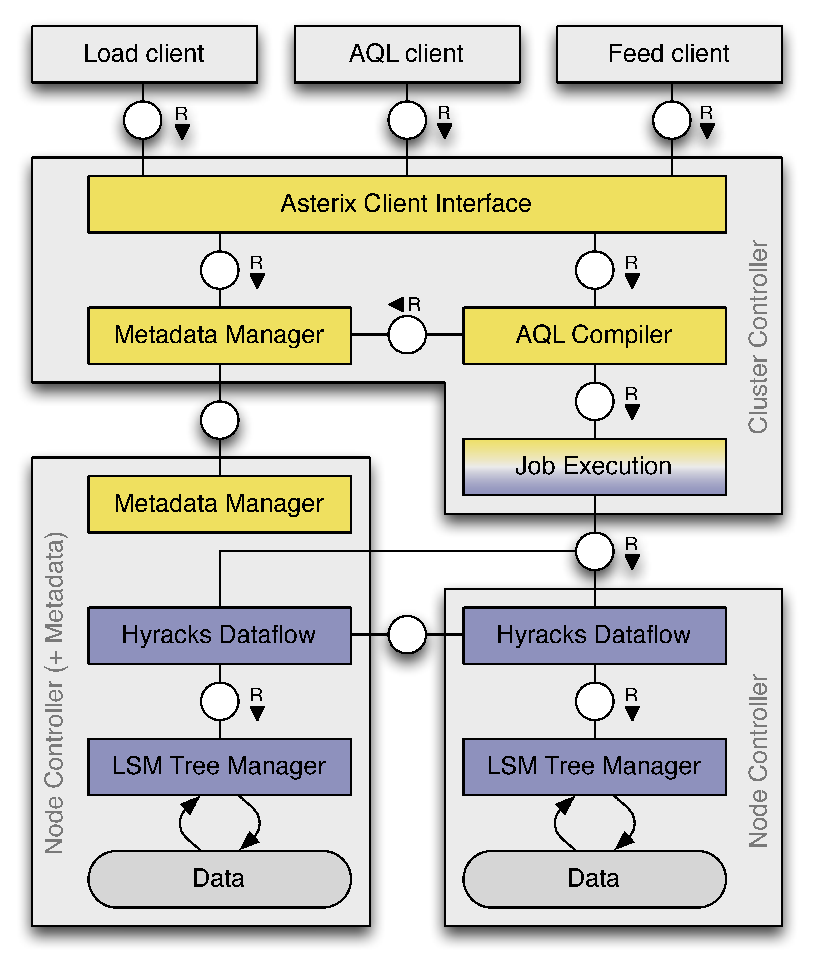
\includegraphics[width=2.7in]{images/asterixdb_arch}
%\vspace*{\betweenfigureandcaption}
\caption{Architecture\label{fig:arch}}
%\vspace{-0.1in}
\end{figure}

This node receives queries via an HTTP-based API and returns their results to the requester either synchronously or asynchronously (in which case a handle to the result is returned and the client can inquire about the query's status and request the result via the handle).
The Query Control Node also runs (a) the AQL compiler that translates AQL statements to Job Descriptions for the dataflow-engine Hyracks and (b) the Job Executor that distributes the Job Descriptions to the Hyracks Node Controllers and starts the execution. The AQL Compiler internally uses Algebricks to compile queries into Hyracks Jobs, that are then executed by the Hyracks Job Executor. Algebricks has access to the Metadata Manager through the metadata interface described in Section~\ref{subsec:metadata} in Chapter~\ref{ch:algebricks}.
The Worker Nodes -- represented by the boxes at the bottom of Figure \ref{fig:arch} -- have to (a) manage their partitions of the data stored in LSM-trees and to (b) run their parts of each Hyracks Job.
In the following subsection we will describe Hyracks and Algebricks. 

\begin{figure}[htb]
\centering
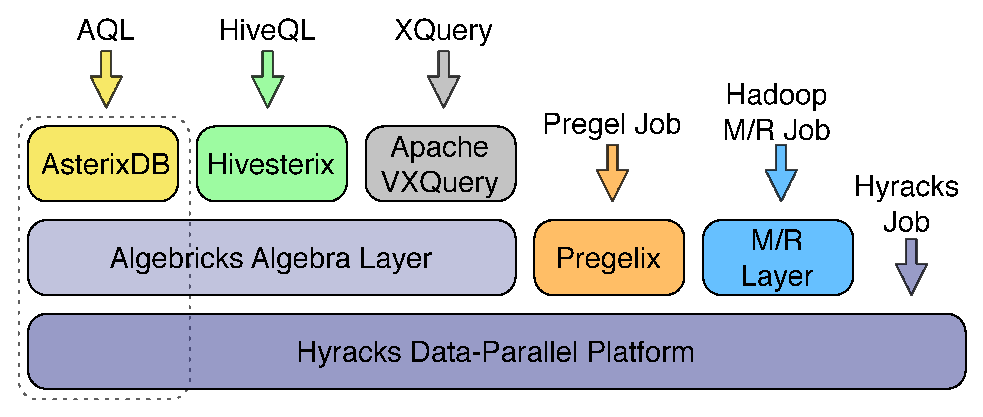
\includegraphics[width=5.0in]{images/asterixdb_stack}
%\vspace*{\betweenfigureandcaption}
\caption{Asterix software stack\label{fig:stack}}
%\vspace{-0.1in}
\end{figure}

\subsection{Hyracks and Algebricks}

The Hyracks layer of AsterixDB is the bottom-most layer of the Asterix software stack as described before, and shown in Figure \ref{fig:stack} repeated here for readability.
Hyracks is the runtime layer (\emph{a.k.a.}~executor) whose responsibility is to accept and manage data-parallel computations requested either by one of the layers above it in the Asterix software stack or potentially by direct end-users of Hyracks. 
In the case of AsterixDB, Hyracks serves as the scalable runtime engine for AQL queries once they have been compiled down into Hyracks Jobs for execution.

As mentioned before, jobs are submitted to Hyracks in the form of DAGs made up of \emph{Operators} and \emph{Connectors}. 
As described in \ref{ch:hyracks}, Hyracks Operators are responsible for consuming partitions of their inputs and producing output partitions. 
Connectors redistribute data from the output partitions and provide input partitions for the next Operator.

Figure \ref{fig:job} depicts the Hyracks Job for Query \ref{q:agg}.
The boxes represent its Operators and the lines represent Connectors.
One thing that we see is that all Connectors, except for the last one, are OneToOneConnectors. 
This means that no redistribution of data is required for this part of the plan---and it can be evaluated on the node that stores the data.
The degree of parallelism (the number of Operator instances evaluating in parallel) for these Operators is the number of partitions that is used to store the Dataset.
Looking at the Operators bottom-up, we see that the first 2 Operators perform a search on a secondary index.
This will return a set of primary key values that are fed into the search Operator on the primary index.
Note that the primary keys are sorted first to improve the access pattern on the primary index.
Above the primary index access we see two Operators that evaluate a predicate that should intuitively always be true for records that were identified by the search on the secondary index. This test is needed owing to the specific record-level transaction model implemented by AsterixDB. For more details about the transaction model supported by AsterixDB, please refer to~\cite{ASTERIX}.
Finally, we see that the \emph{avg} function that encapsulates the rest of the query has been split into two Operators: a \emph{Local Aggregation Operator} that pre-aggregates the records for the local node and a \emph{Global Aggregation Operator} that aggregates the results of the the Local Aggregation Operators.
Between these Operators is a MToNReplicatingConnector.
As the degree of parallelism for the Global Aggregation Operator is constrained to be 1, the Connector replicates the results of all instances of the Local Aggregation Operators to the single instance of the Global Aggregation Operator.
This split maximizes the distributed computation and minimizes network traffic.

\begin{figure}[htb]
\centering
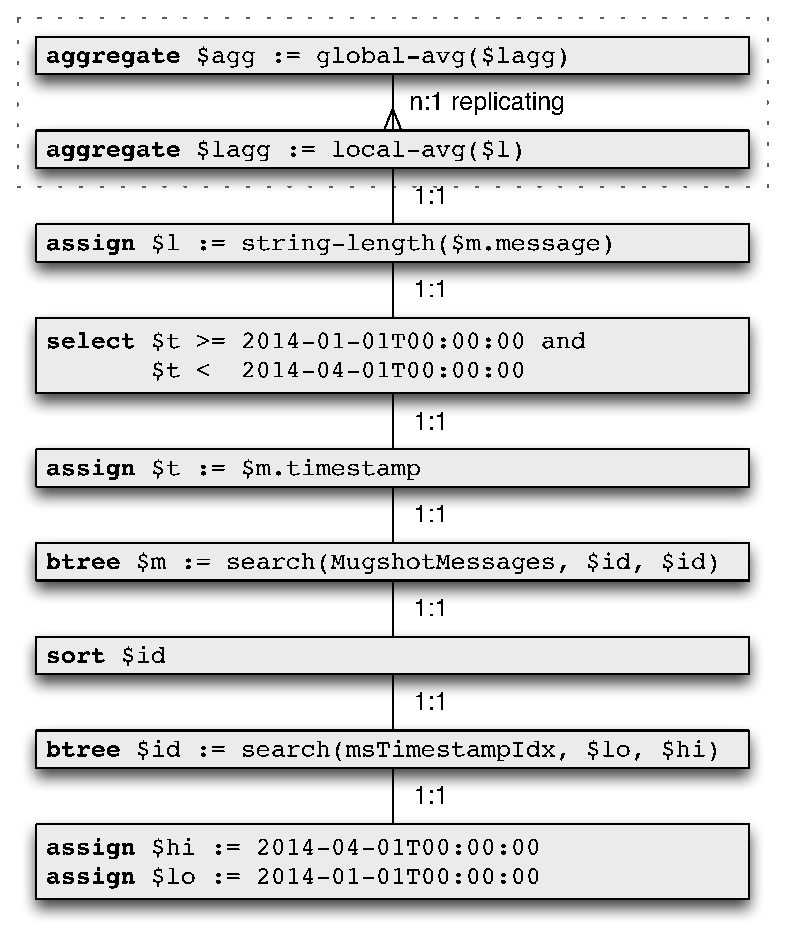
\includegraphics[width=3.0in]{images/hyracks-job2}
%\vspace*{\betweenfigureandcaption}
\caption{Hyracks job of the aggregation query in Query~\ref{q:agg}\label{fig:job}}
%\vspace{-0.1in}
\end{figure}

As the first step in the execution of a submitted Hyracks Job, its Operators are expanded into their constituent \emph{Activities}. 
While many Operators have a single Activity, some Operators consist of two or more Activities.
For example, a HybridHash Join Operator is made up of two Activities, the Join Build Activity and the Join Probe Activity. 
This expansion is made possible by APIs that Hyracks provides to Operator implementors to enable them to describe such behavioral aspects of an Operator.
Although Hyracks does not understand the specifics of the various activities of an Operator, exposing the blocking characteristics of Operators provides important scheduling information to Hyracks -- the separation of an Operator into two or more Activities surfaces the constraint that it can produce no output until all of its input has been consumed.

To execute a Job, Hyracks analyzes the Activity graph produced by the expansion described above to identify the collections of Activities (Stages) that can be executed at any time (while adhering to the blocking requirements of the Operators). 
Each Stage is parallelized and the resulting graph is executed in the order of the dependencies. 
More details about Hyracks' computational model, as well as its implementation and performance, are available in \cite{hyracks}.

The Hyracks job shown above, is generated by the Algebricks layer in AsterixDB. AsterixDB's AQL parser parses the query (Query~\ref{q:agg}, in this case) and produces a logical query expression using Algebricks operators, shown in the listing below.

\lstset{numbers=left, numberstyle=\tiny, stepnumber=1, numbersep=5pt}
\begin{center}
\scriptsize
\begin{lstlisting}
DISTRIBUTE-RESULT( $$temp1 )
PROJECT $$temp1
AGGREGATE $$temp1: avg( $$temp0 )
ASSIGN( $$temp0:string-length(
    field-access-by-name($$m, "message")) )
SELECT( algebricks-and(
    algebricks-ge(field-access-by-name($$m, "timestamp"), 
        datetime("2014-01-01T00:00:00")), 
    algebricks-lt(field-access-by-name($$1, "timestamp"), 
        datetime("2014-04-01T00:00:00")) )
UNNEST( $$m:dataset("MugshotMessages") ) 
EMPTY_TUPLE_SOURCE
\end{lstlisting}
\end{center}

After the initial logical plan is created, the compilation of the query proceeds using the Algebricks compiler. The metadata provider implemented within AsterixDB exposes source metadata to the Algebricks compiler. In the example above, the metadata provider is used to check if ``MugshotMessages'' is a valid dataset, and if so, also fetch the type associated with this dataset. In this specific instance, Algebricks realizes that the dataset has a secondary index on the ``timestamp'' field, and hence the time-range selection can be achieved by using that index. Based on this information, the Algebricks compiler rewrites the bottom part of the logical expression into one that would use the secondary index. Furthermore, Algebricks also optimizes the aggregate step of the query by converting it into a two-step distributed aggregate operation so that the amount of data transported over the network is minimized. The rewrite rule that utilizes indexes is specific to AsterixDB and lives in the AsterixDB codebase. On the other hand, the rule that optimizes aggregation for parallelism is available as part of the core Algebricks distribution.

AsterixDB uses the Algebricks framework to perform some optimizations specific to itself. As mentioned before, AsterixDB supports open types. A field accessed in a record of an open type might fall under one of two categories. The field could be one that was defined in the open type definition of the record type, or it could be a non-declared field. The concrete datamodel representation of record values in AsterixDB stores these two types of fields in different ways. Declared fields are stored without storing their field names in every record instance, and can be accessed using the index of the field. The undeclared fields, on the other hand, are stored along with their name. Although the declared fields can be accessed by name (by first probing the record type definition for the index, and then accessing the actual field value in the record instance by index), it is more efficient to ``constant-fold'' the name-to-index mapping step, so that the field can be looked up directly by index at runtime. AsterixDB uses a rewrite rule to perform data-flow analysis at compile-time to identify type lineage of values to maximize the locations in the query where the name-to-index mapping can be performed during compilation. All such occurrences of ``field-access-by-name'' invocations are then replaced by the ``field-access-by-index'' function, thus making the cost of accessing declared fields no worse than the costs associated with accessing fields in a fully typed language like SQL.

\section{Conclusion}

In this chapter, we took a look at AsterixDB, a semi-structured, parallel Big Data Management System and the roles of Hyracks and Algebricks in its architecture. Hyracks and Algebricks form core foundational pieces that provide significant functionality for compiling AQL queries and then running them in parallel on commodity clusters.
